\documentclass[12pt]{article}

\usepackage[a4paper, margin=2.5cm]{geometry}
\usepackage{graphicx}
\usepackage{rotating}
\usepackage[english]{babel}
\usepackage{appendix}
\usepackage{listings}
\usepackage{url}
\usepackage{todonotes}

\graphicspath{{./resources}}
  
\title{COMP3900-H15A-capSquad - Project Proposal}
\date{\today}
\author{Daniel Latimer z5115175 \\ Connor O'Shea z5115177 \\ Kevin Chan z5113136 \\ Oliver Richards z5157383 \\ Peter Kerr z5115807} 

\begin{document}

\maketitle
\tableofcontents
\newpage

\section{Background}

\begin{figure}
    
\includegraphics[width=\textwidth]{resources/spongebob}
    \caption{Background? \cite{Laird2012}}
    \label{fig:background}
\end{figure} \todo{delete me}

\subsection{Problem Domain}
\subsection{Existing Systems}

%\section{Project Objectives} % May not be necessary

\section{User Stories}
\subsection{Product Backlog}
\subsection{Project Objectives}
\subsection{Novel Features}

\section{Sprints}
% Must have:
%   - Start + end dats of all sprints
%   - User stories in 1st sprint
%   - 

\section{Interface and Flow Diagrams}

\section{System Architecture}

% Talk about the data/business/presentation layers
% Talk about the external actors
% 3rd party technologies used

\begin{figure}
    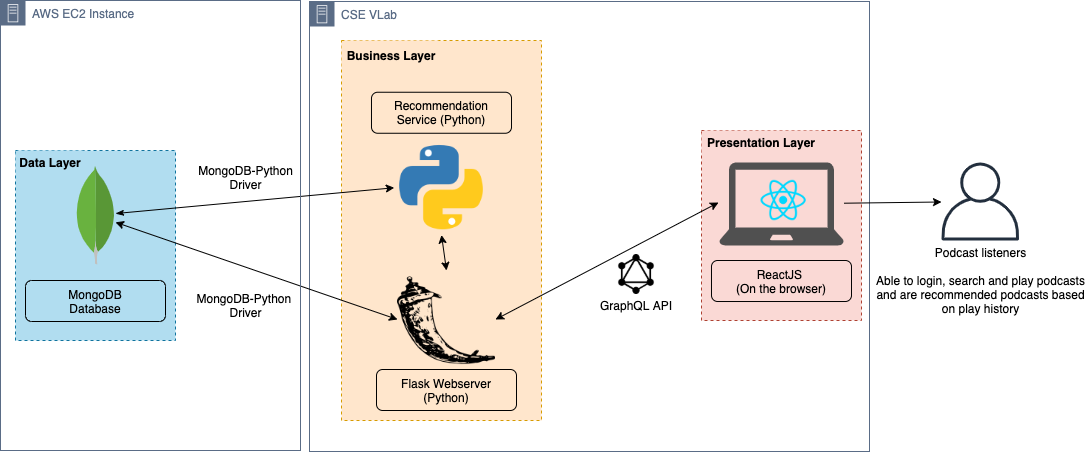
\includegraphics[width=\textwidth]{resources/SystemArchitecture}
    \caption{Proposed System Architecture}
    \label{fig:SysArch}
\end{figure}

\bibliography{library.bib}
\bibliographystyle{plain}
\end{document}
